This chapter presents a detailed explanation of the neural network models proposed in this work and
the correspondent baselines used for comparison. In section one the architectures of
the main networks are shown. In section 2 the loss functions used are described. Finally,
section 3 shows the baselines models used for the ablation study of both performance and
explainability.

\section{Network architectures}
As was mentioned before, the main principle followed for model design is to enhance explainability
while maintaining performance as much as possible. With that in mind, we combine two
state of the art techniques from the deep learning literature, semantic segmentation
and attention mechanisms to design three novel architectures that present a significant
improvement in explainability over traditional blackbox CNNs. We describe these architectures
in the following sub sections, ordered by model complexity.

\subsection{Segmentation as a feature extractor.}
The traditional deep learning approach in computer vision, consists of using a pretrained
CNN \cite{lecun_mnist}, on the Imagenet dataset \cite{imagenet}, such as the ResNet \cite{he_resnet},
usually called the feature extractor, and then stacking a custom set of layers over its output features. Leaving the CNN weights
fixed or updating them on training  depends on the particular problem. This is the approach taken
by most of the previous literature on urban perception \cite{hidalgo_placepulse,tamara_judgments,zhang_measuring}.

In this work, we propose replacing the traditional feature extractors for a fully trained semantic segmentation
network. The semantic segmentation task consists of assigning a label to every pixel in an image, and therefore
it implies a fine grained detection of object edges, providing a rich amount of information that is human understandable.
The output of a semantic segmentation model is a probability distribution over the different classes for each pixel,
making it usable as a feature map of the image. See figure \ref{fig:segmentation} for an example.

We base our models on the PSPNet architecture \cite{pspnet}, since it is one of the highest performing models
available in the literature. It's design its based on a ResNet50 and a pyramid pooling module, which consists on
parallel poolings and convolutions at different scales, that are then concatenated and used to generate the output with a
final convolution and a softmax layer.

\begin{figure}[ht]
	\begin{center}
	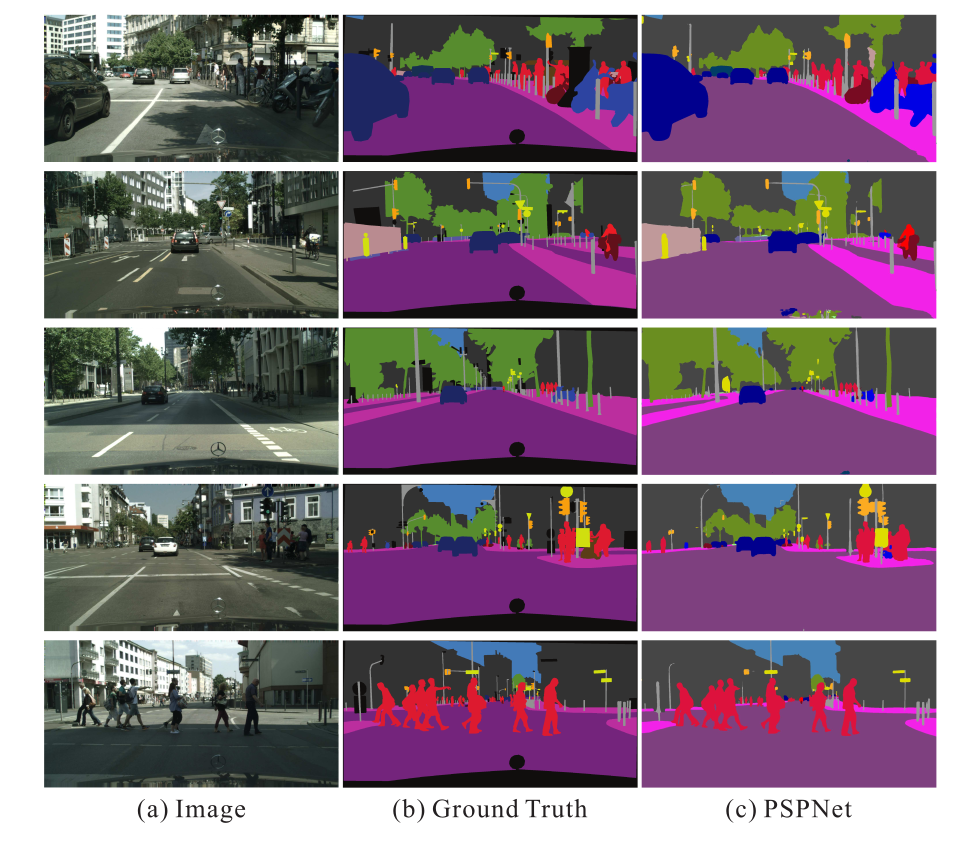
\includegraphics[width=0.8\textwidth]{./figures/segmentation.png}
	\caption[Example of Semantic Segmentation]{Examples of semantic segmentation by the PSPNet model on the CityScapes dataset. Extracted from \citeA{pspnet} }
	\label{fig:segmentation}
	\end{center}
\end{figure}

\begin{figure}[ht]
	\begin{center}
	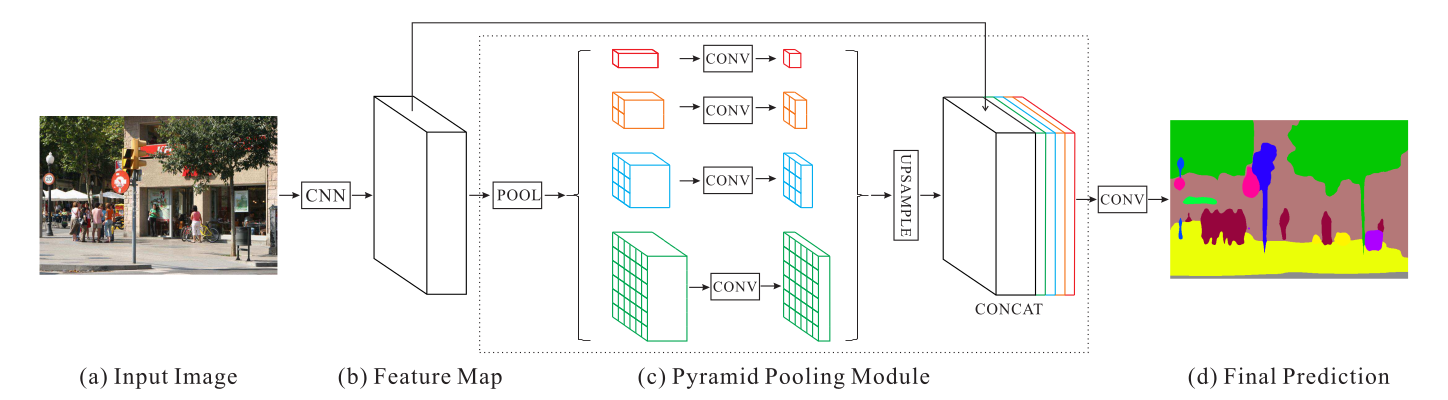
\includegraphics[width=0.9\textwidth]{./figures/pspnet.png}
	\caption[PspNet architecture]{PSPNet architecture. Extracted from \citeA{pspnet} }
	\label{fig:segmentation}
	\end{center}
\end{figure}


We train PspNet on the CityScapes dataset \cite{cordts_cityscapes}, since its urban images taken from a car have
considerable similarity to street view images, and its classes have proven informative for the urban perception problem
in previous research \cite{rossetti,zhang_measuring}.  After this process we keep the network weights fixed
and use the output as a features for subsequent layers.

\subsection{Self attention.}

\subsection{Segmentation as attention query.}

\section{Loss function}

\section{Baselines}

\subsection{ResNet50 + MLP}

\subsection{ResNet50 + Attention layers + MLP}